%!TEX root = ../../../adrien_gomar_phd.tex

A single-blade passage meshed
with an O4H topology is used to compute this
CROR configuration as show in Fig.~\ref{fig:dream_mesh}. This is a classical
topology for turbomachinery computations that is here applied to 
a CROR.
\begin{figure}[htp]
  \centering
  \subfigure[Topology]{
    \label{fig:dream_mesh}
    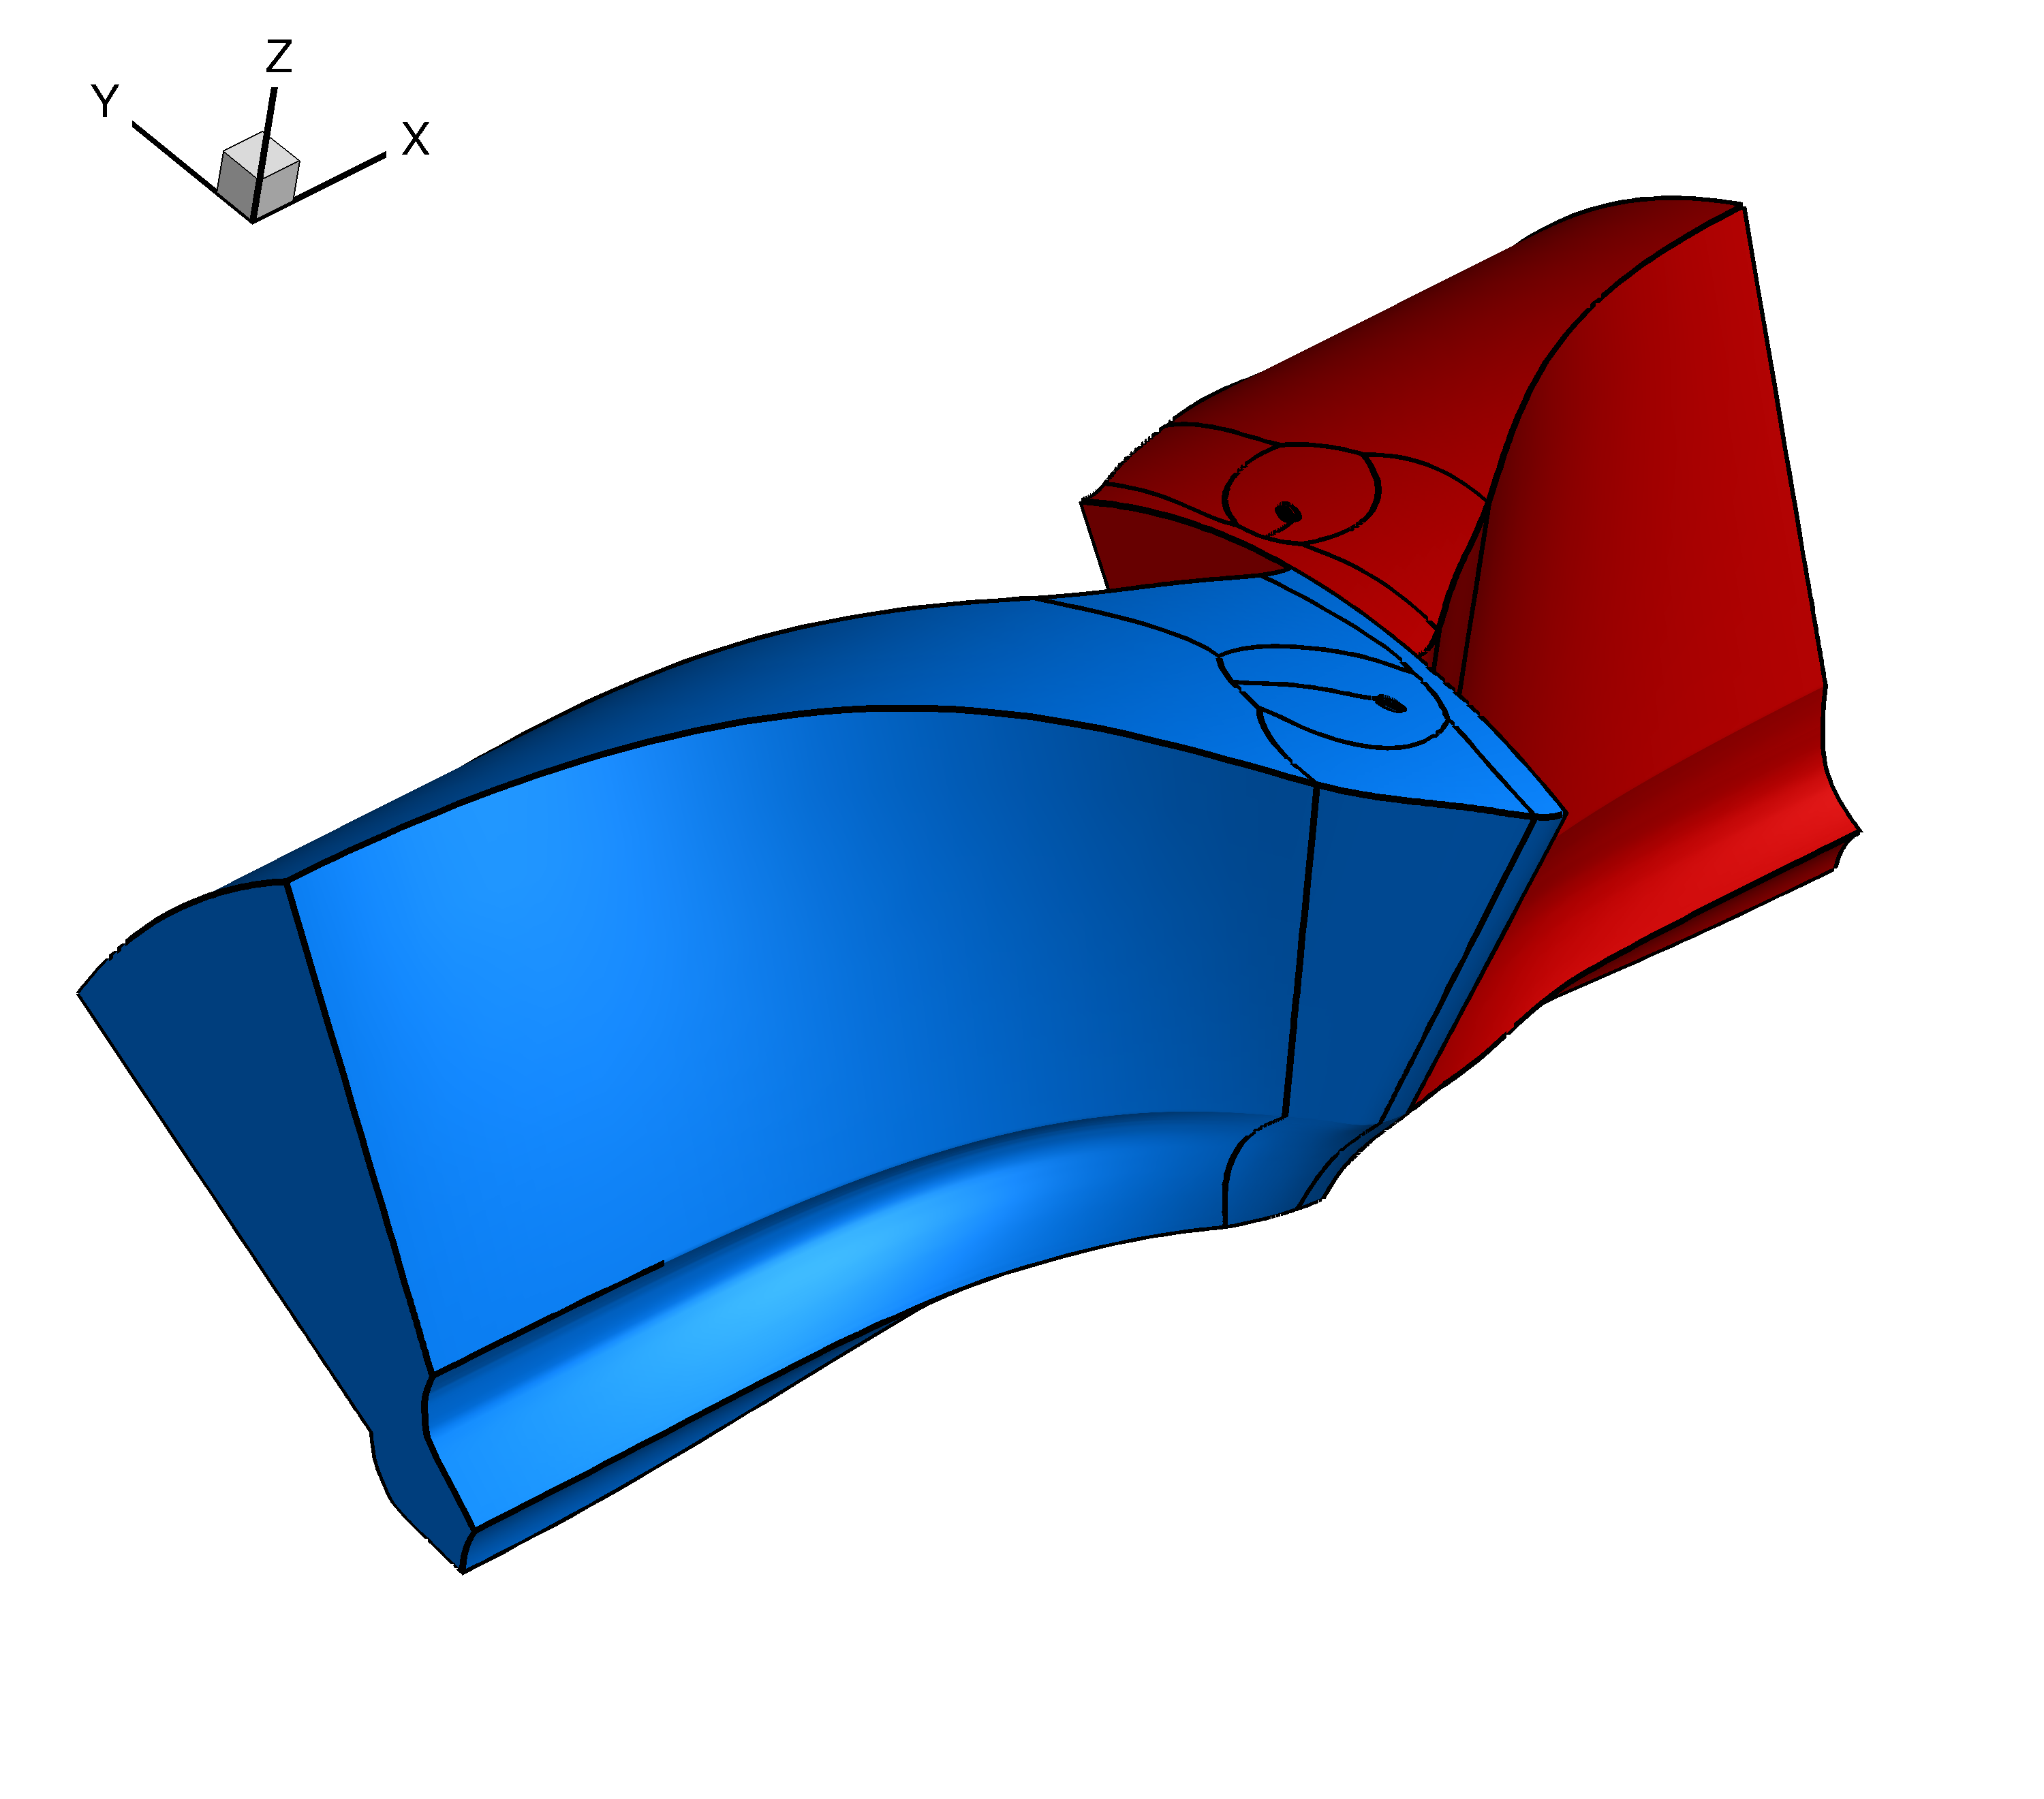
\includegraphics[height=.4\textwidth]{dream_mesh.png}}
  \subfigure[Detailed topology with number of grid points]{
    \label{fig:dream_ls_mesh}
    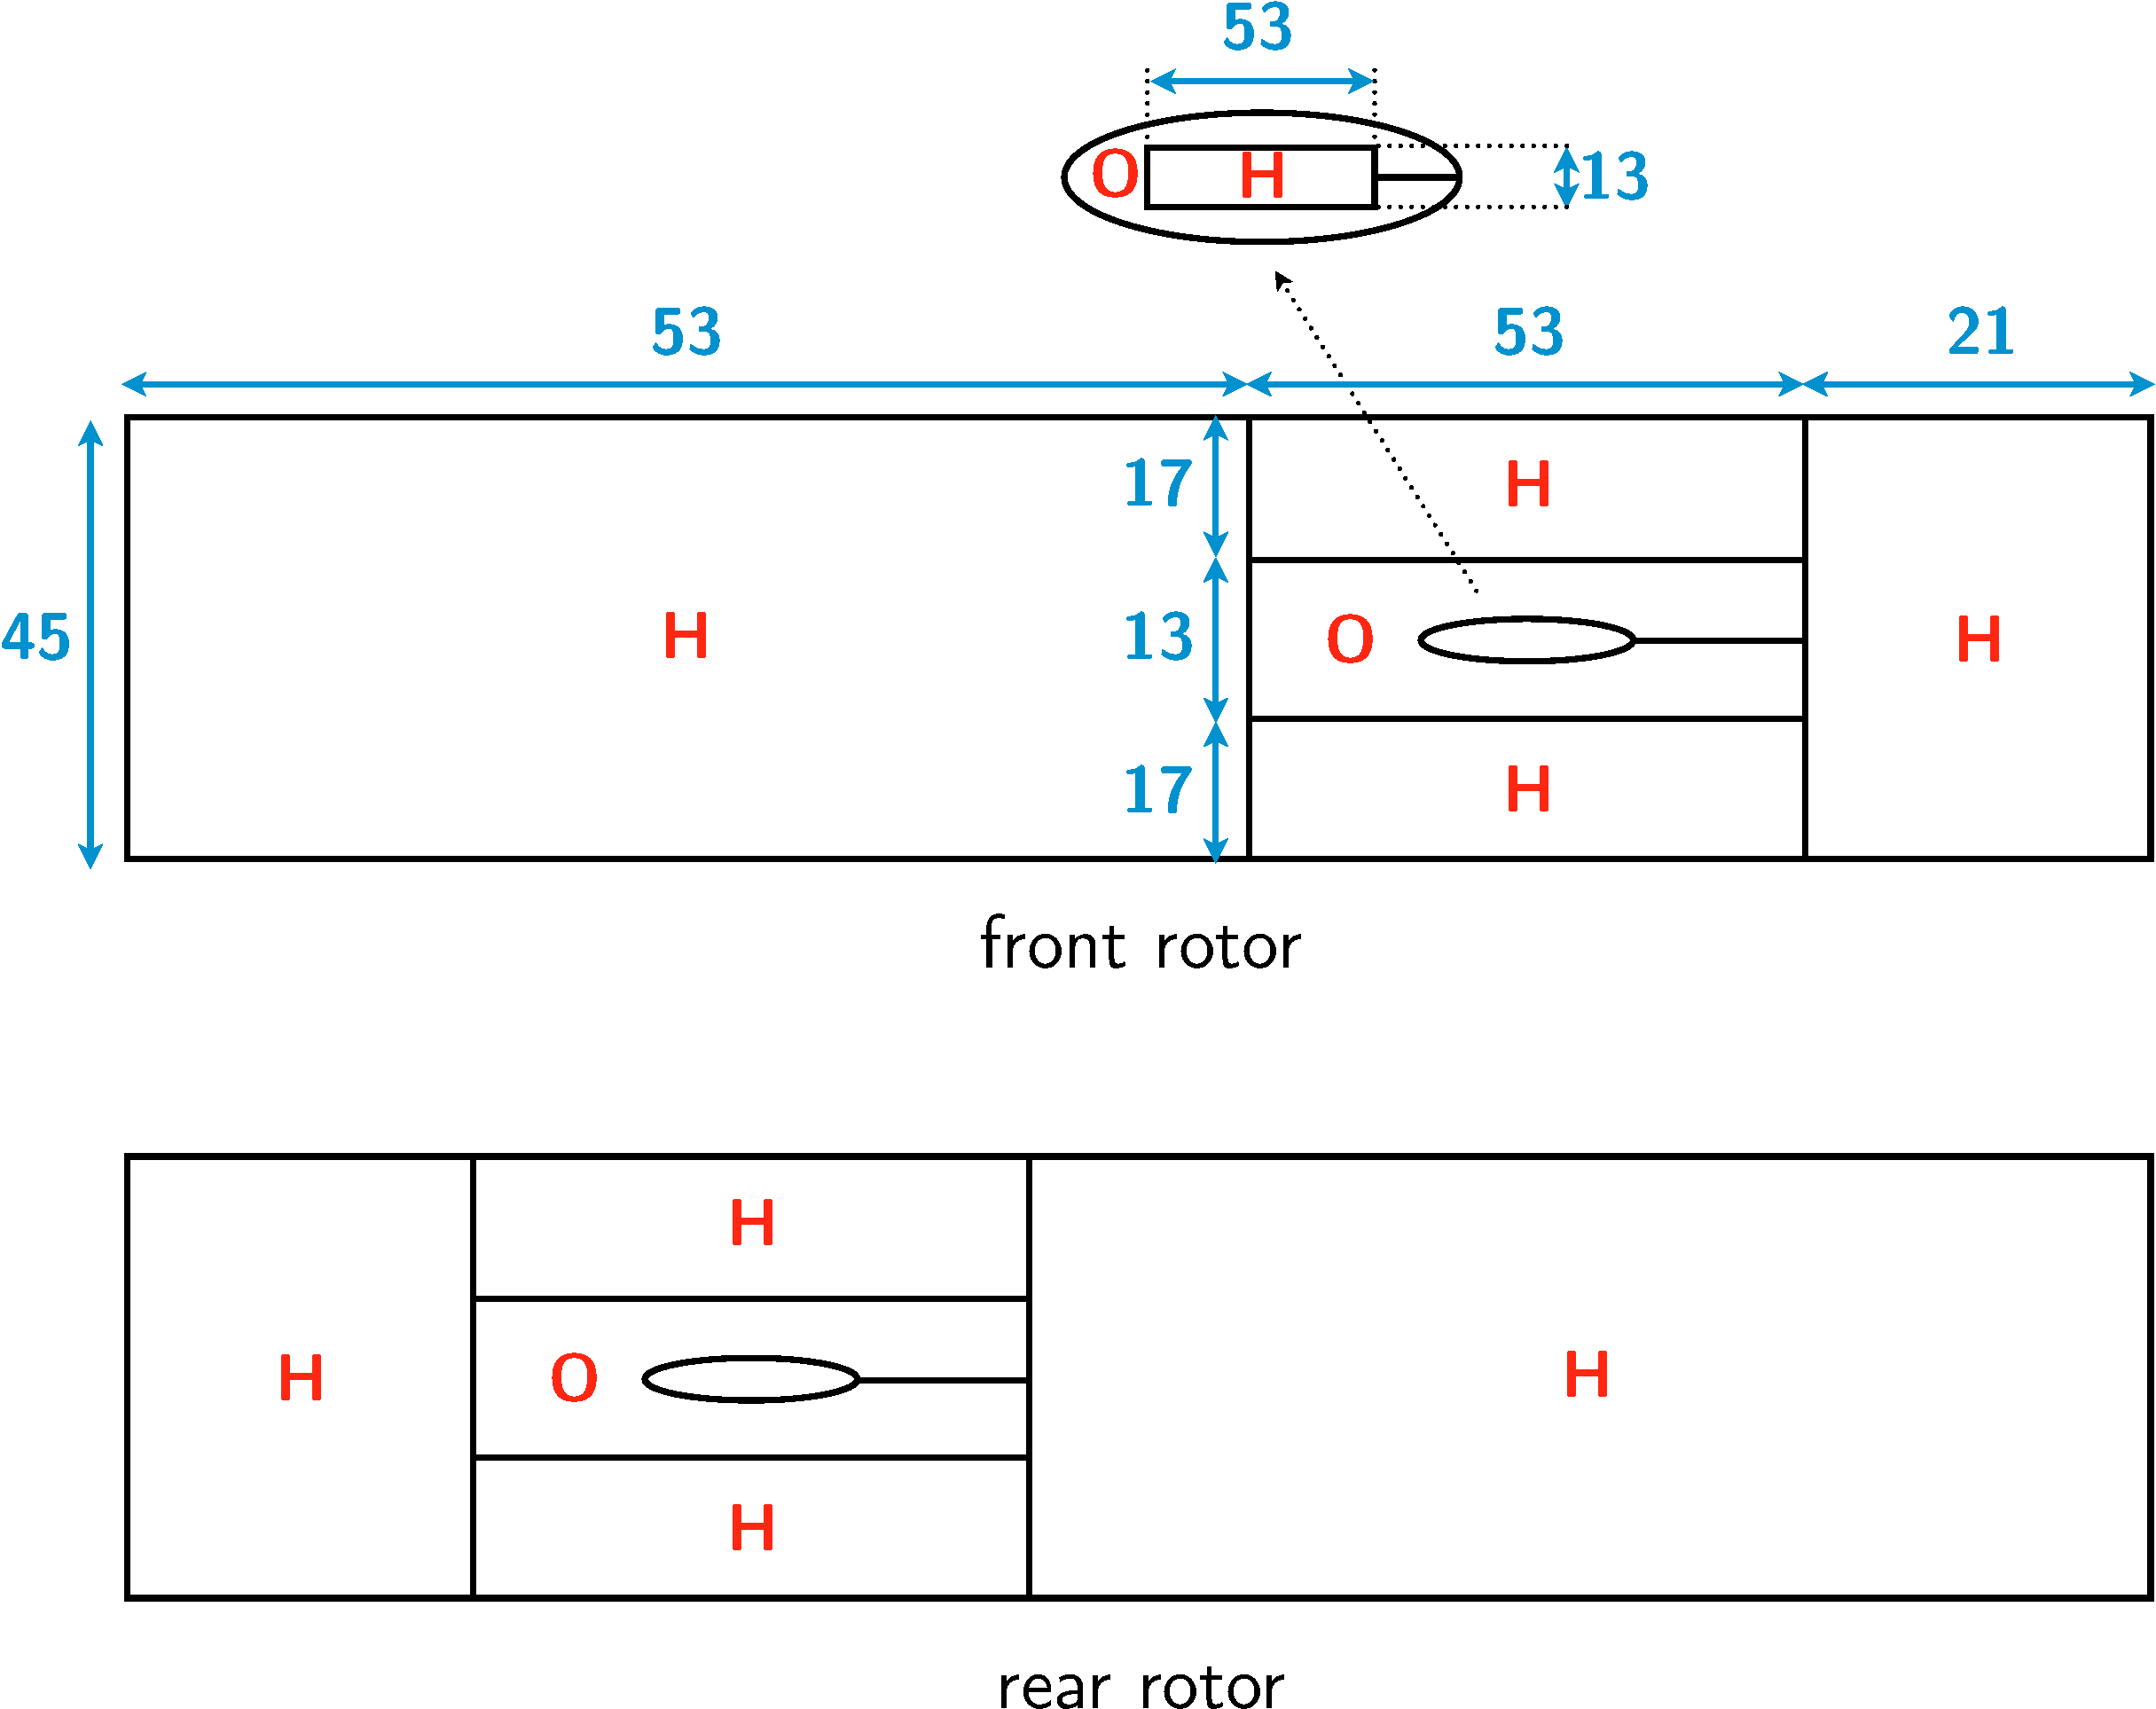
\includegraphics[height=.4\textwidth]{dream_ls_mesh.pdf}}
  \caption{Low-speed isolated configuration mesh topology.}
\end{figure}
The number of points is reported in 
Fig.~\ref{fig:dream_ls_mesh} for a blade-to-blade section. 
129~points discretize the blade, 45~the pitch and 181~the radial
extent. The same number of points is used for the front
and the rear rotors. 
Finally, the total number of grid points is almost $5$ million, which
is consistent with the literature~\cite{Stuermer2008,Bechet2011,
Francois2013,Zachariadis2011,Peters2012}.

As a CROR is not shrouded, a sufficiently large
far-field domain is taken to ensure a minimum influence
of the far-field boundary conditions on the results.
The computational domain is shown in Fig.~\ref{fig:dream_farfield}.
The radial extent is $3D$ while the axial one is $3.5D$, with
$D$ being the diameter of the front rotor.
In the literature, 
\citet{Peters2012} consider an axial extent of $7.5D$
with a radial extent of $4D$ while \citet{Zachariadis2011}
consider $2.5D$ and $3.6D$, respectively. We are thus in 
the mid-range of the values taken in the literature.
\begin{figure}[htp]
  \centering
  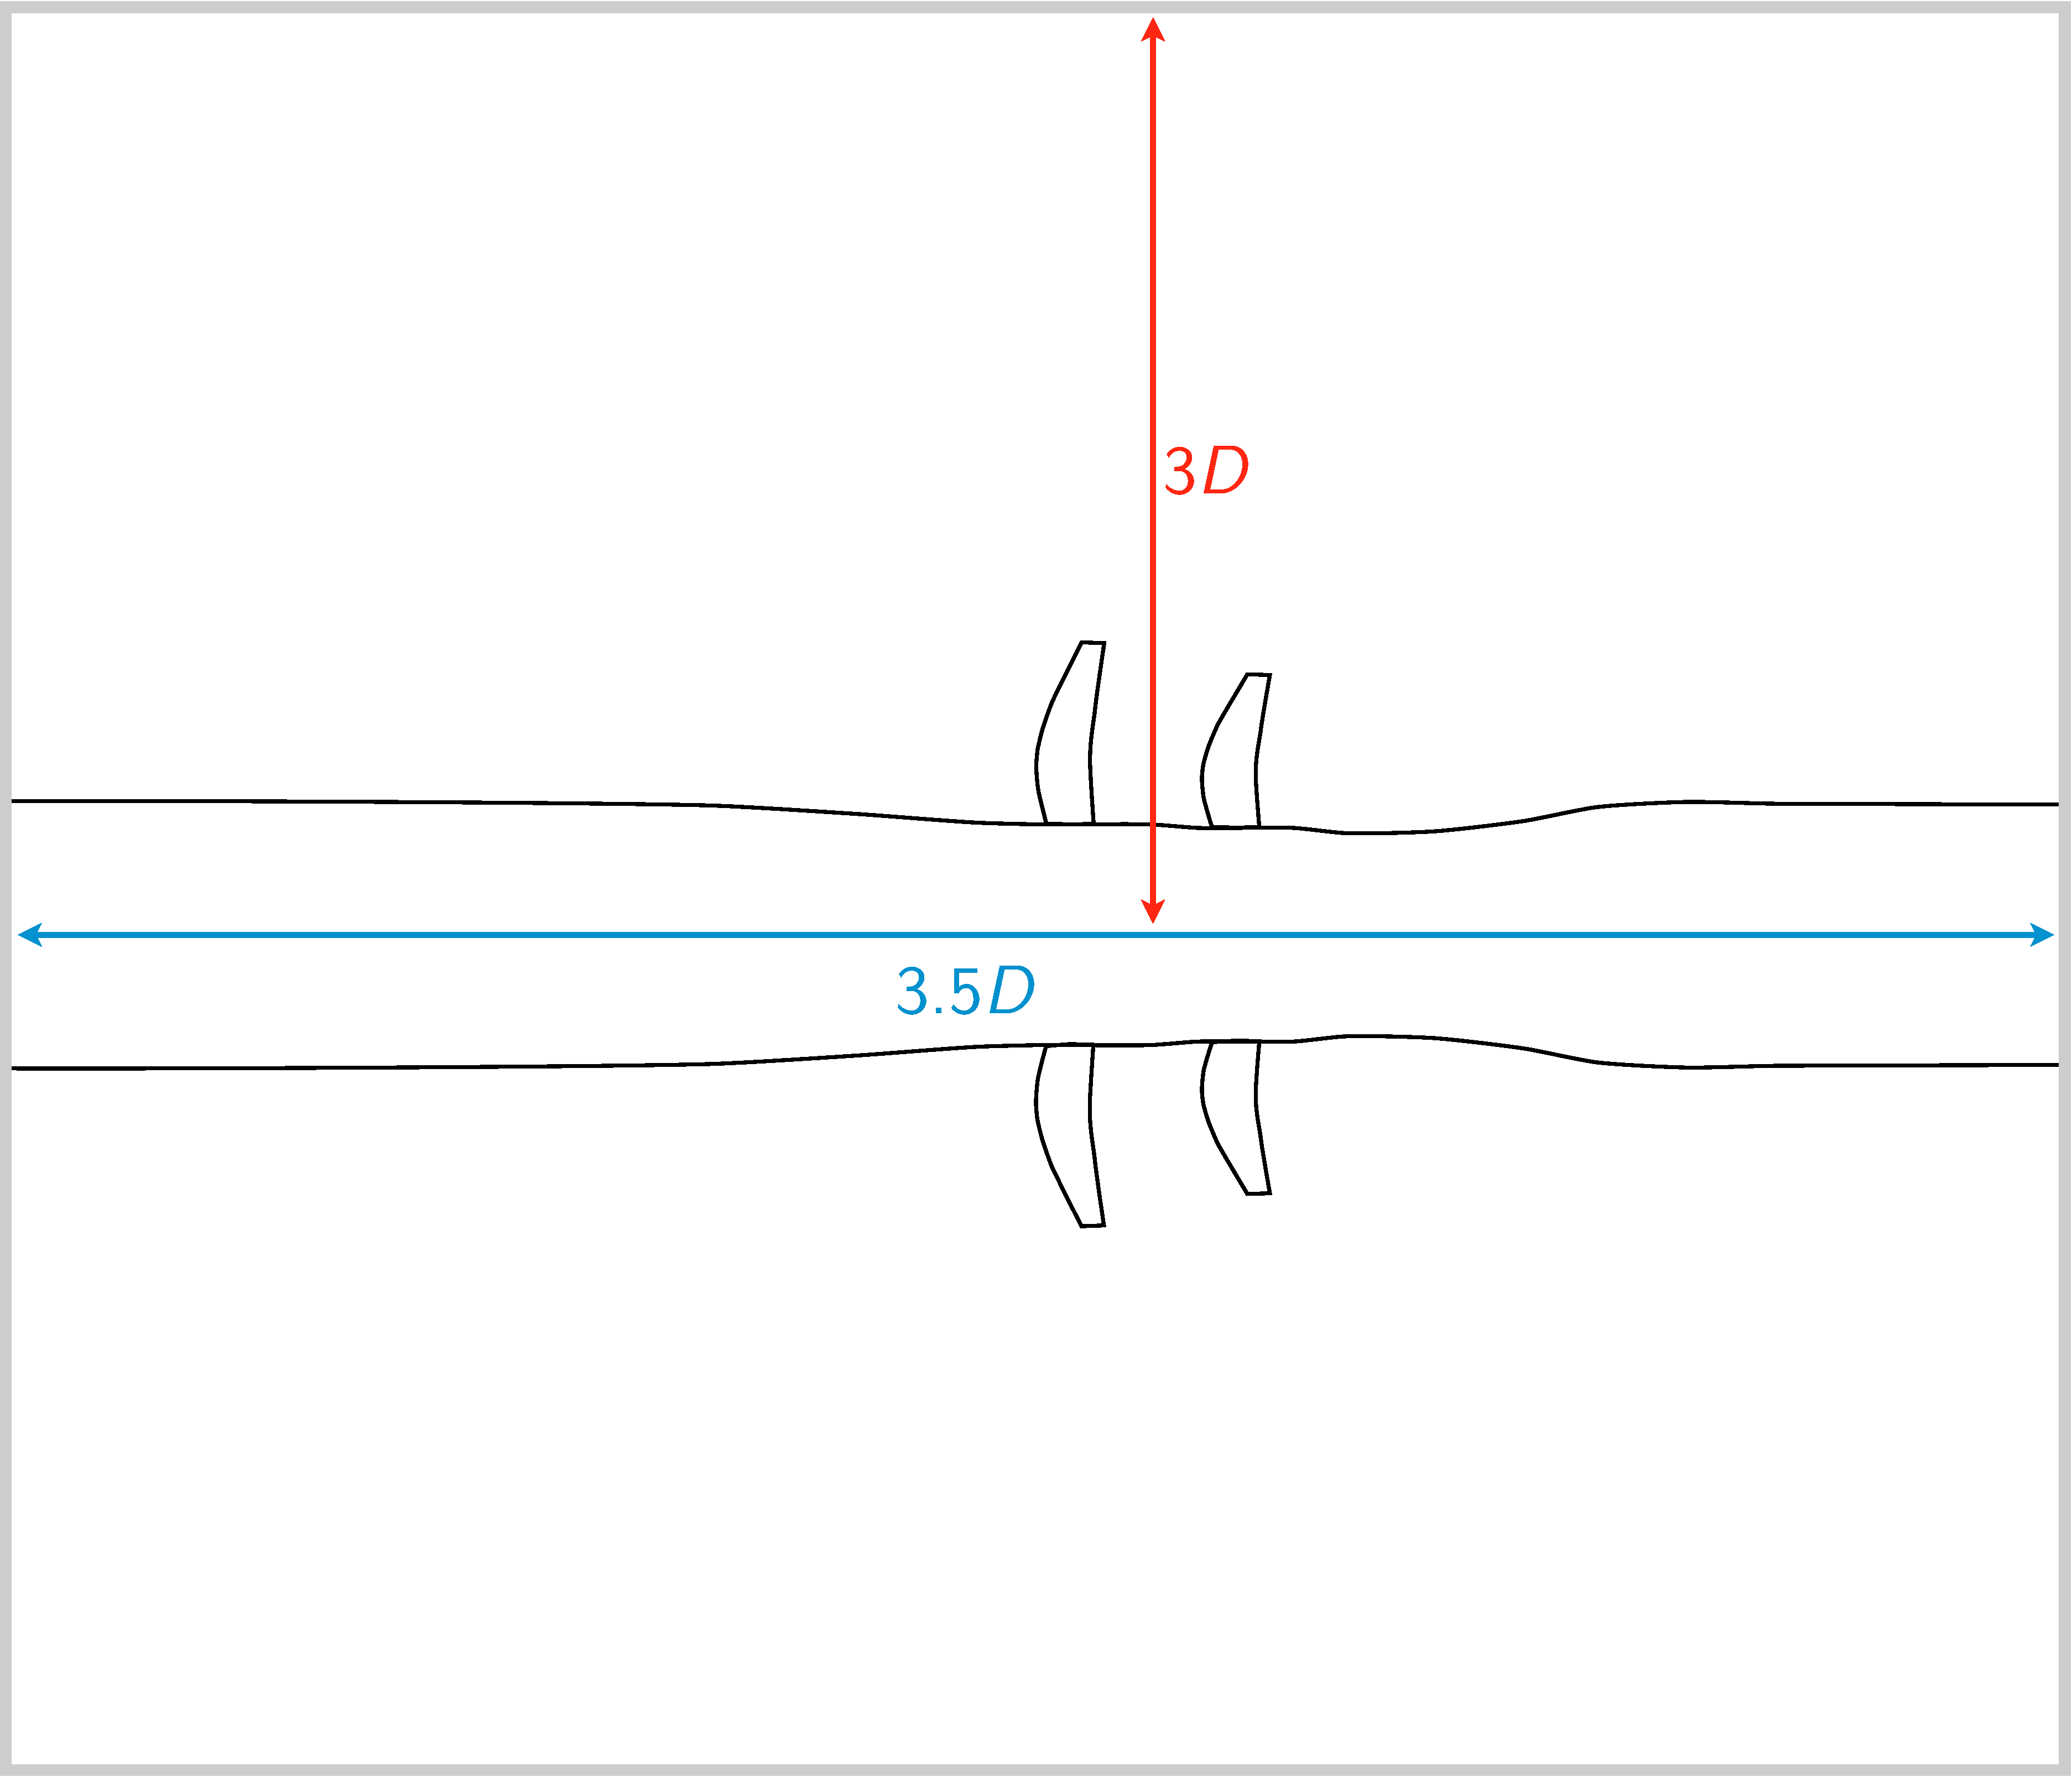
\includegraphics[width=.4\textwidth]{dream_farfield.pdf}
  \caption{Low-speed isolated configuration far-field domain and boundary conditions.}
  \label{fig:dream_farfield}
\end{figure}
As highlighted by the underlined text in Fig.~\ref{fig:dream_farfield},
the boundary conditions used here are: (i)~adiabatic walls
for the blades and the shroud (or spinner), (ii)~constant
stagnation values used at the far-field, (iii)~periodic
or phase-lagged for the azimuthal boundaries of the channel
and (iv)~a mixing-plane or a sliding mesh interface is
used depending on the type of computation (steady or unsteady).
In opposite to the mesh convergence study made previously on the STCF11
configuration (see Sec.~\ref{sec:stcf11_numerical}),
the mesh stems from literature and industrial best
practices and will thus not be assessed.

Turbulence is modeled using the one-equation model of
\citet{Spalart1992}.  Roe's scheme~\cite{Roe1981} along with a 
second-order MUSCL extrapolation 
is used to compute the convective fluxes.
The maximum CFL number is set to~10 for the steady 
computations and to~5 for the unsteady simulations.

\paragraph{Influence of the spatial discretization}
\label{sub:dream_ls_spatial_discretization}

To assess the influence of spatial discretization, four 
space schemes are used to simulate the low-speed CROR configuration.
These four schemes are the \citet{Jameson1981} scheme (noted JST) with artificial
viscosities $\kappa_4 = 0.016$, $\kappa_4 = 0.032$, $\kappa_4 = 0.064$
and $\kappa_2$ equal to $0.5$ as the operating point (Low-speed
flight condition) should not 
lead to shocks. In addition to this scheme, three upwind
Roe's schemes~\cite{Roe1981} along with no extrapolation (noted Roe~1),
a second order (noted Roe~2) or a third-order (noted Roe~3) 
MUSCL extrapolation are used.

The convergence of the different computations is show 
in Fig.~\ref{fig:dream_ls_space_scheme_residual}
for the four schemes. The convergence is not 
very good. Only the Roe~1 and Roe~2 spatial schemes give 
a convergence that has an acceptable slope. In contrary,
the JST~$\kappa_4 = 0.016$ diverges and the three
remaining schemes hardly converge. The higher the
viscosity parameter $\kappa_4$ of the JST scheme, the better
the convergence. Exceeding $\kappa_4 = 0.064$ should
warn us that something might be wrong with the computation.
As stated previously, this is actually due to the range of Mach
number in which this low-speed configuration operates. In fact,
a part of the computation can be said to be within the incompressible
range ($M \leq 0.3$) and therefore not adapted to a compressible
flow solver which is the case of the \emph{elsA} code 
(see Appendix~\ref{app:elsa}).
\begin{figure}[htp]
  \centering
  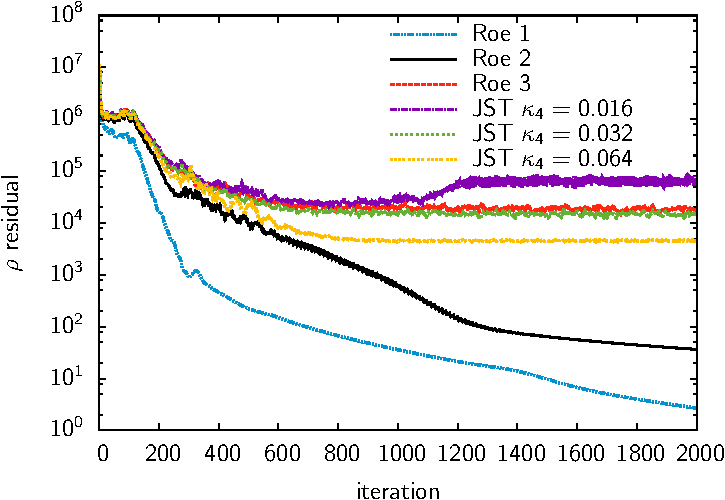
\includegraphics[width=.5\textwidth]{SPACE_SCHEME_DIFF_LS_RESIDUALS.pdf}
  \caption{Low-speed isolated configuration: convergence of 
  steady computations using different spatial schemes.}
  \label{fig:dream_ls_space_scheme_residual}
\end{figure}

To further differentiate the spatial schemes, 
the steady results for the similarity coefficients are reported
in Fig.~\ref{fig:dream_ls_space_scheme_coeff} for all spatial scheme, 
except the diverging JST~$\kappa_4 = 0.016$ computation.
The results are normalized by the Roe~2 values.
The Roe~2, Roe~3, and the two JST schemes give equivalent
similarity coefficients as the difference is smaller than 1~\%.
In opposite, the first order upwind scheme Roe~1 give a 5~\%
difference for both the traction coefficient $C_T$ and the efficiency $\eta$.
Cross-comparing these results with the convergence of the computations
reported in Fig.~\ref{fig:dream_ls_space_scheme_residual}, the Roe~2
scheme is kept for the following as it give both a good convergence
of the residuals and consistent similarity coefficients.
\begin{figure}[htp]
  \centering
  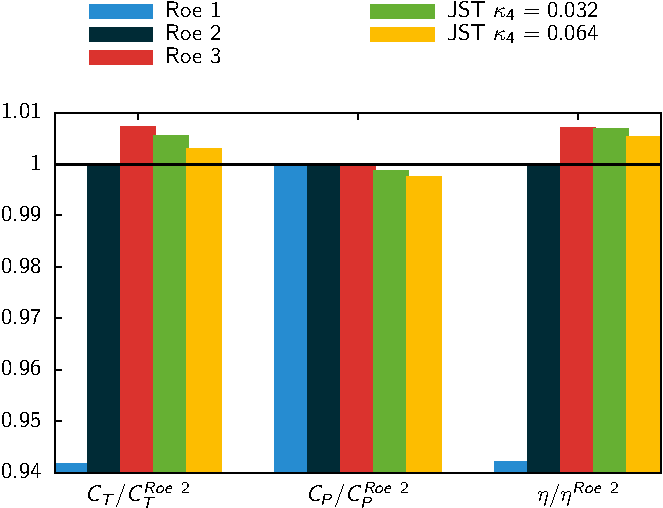
\includegraphics[width=.5\textwidth]{SPACE_SCHEME_DIFF_LS_COEFF.pdf}
  \caption{Low-speed isolated configuration: convergence of 
  similarity coefficients using different spatial schemes.}
  \label{fig:dream_ls_space_scheme_coeff}
\end{figure}
